\documentclass{article}

\usepackage{iclr2026_conference,times}
\input{math_commands.tex}

\usepackage{amsmath}
\usepackage{amssymb}
\usepackage{booktabs}
\usepackage{graphicx}
\usepackage{hyperref}
\usepackage{microtype}
\usepackage{tabularx}
\usepackage{url}
\usepackage{xcolor}

\hypersetup{hidelinks}
\graphicspath{{../figures/}}

\title{When Plausible Videos Lie:\\Action-Consistency Audits for Video Futures}

% The ICLR submission style hides this block while \iclrfinalcopy remains commented.
\author{Anonymous authors\\Paper under double-blind review}

\newcommand{\nset}{\{1,2,4,8,16,32,64\}}
\DeclareRobustCommand{\resultfile}[1]{\nolinkurl{#1}}
\newcommand{\score}{s}
\newcommand{\utility}{u}
\newcommand{\selected}{\mathrm{sel}}
\newcommand{\gate}{Action-Consistency Gate}

%\iclrfinalcopy

\begin{document}
\maketitle

\begin{abstract}
Generated video futures are persuasive planning objects: they look like outcomes, not merely scores. This paper audits a selected-tail failure mode in which a visually smooth, goal-like future is not faithful to the actions that supposedly caused it. In a controlled action-conditioned RGB grid world, large candidate-count visual selection increasingly chooses videos that cross a hidden wall or emerge from an occluder without a valid action-conditioned path. The original four-artifact suite shows that from candidate count \(1\) to \(64\), selected visual plausibility increases by \(0.072\) while executed utility falls by \(1.52\), and a three-seed check gives a mean utility drop of \(1.90\). The expanded suite extends raw selection to \(N=256\): visual plausibility rises by \(0.077\), action-consistency violation rises by \(0.484\), and real executed utility falls by \(1.946\). A calibrated video repair and a direct action-consistency filter each improve \(N=256\) executed utility by \(4.600\) in the controlled world. We contribute a counterfactual video benchmark, a tie-aware finite-pool selection law, video-specific diagnostics, score-key and occlusion stress tests, and a scoped repair gate using action consistency, temporal causality, occlusion uncertainty, frame-state agreement, and small held-out calibration. The claim is intentionally bounded: this is a controlled warning and audit protocol for action-conditioned video futures, not evidence of broad deployment validity or benchmark dominance.
\end{abstract}

\section{Introduction}

Generated video futures are compelling because they show what might happen rather than merely assigning a value to it. This makes them attractive for model-based control, offline planning, and reranking: sample candidate futures conditioned on actions, score the imagined videos, and choose the best-looking rollout. The same visual concreteness can also hide a failure. A video can look smooth, goal-reaching, and temporally plausible while no longer being faithful to the actions that supposedly caused it.

The problem is not only that learned dynamics can be wrong. The sharper concern is selected-tail amplification. If a planner samples many futures and selects the one with the highest internal video score, the selected future is drawn from the score tail. A visually plausible but action-invalid tail may be rare under the generator, yet become common under top-score selection. Increasing the inference budget can therefore make the selected video look better while making the attached action sequence execute worse.

This paper isolates that failure in a controlled setting. The environment is an \(8 \times 8\) grid rendered into RGB video frames. The agent begins left of a vertical wall, the goal lies to the right, and a grey occluder covers the visually tempting crossing region. The real dynamics block the direct path. A generated future may nevertheless show the agent smoothly passing through the hidden wall, then reaching the goal. If the scorer rewards visual smoothness, directness, goal-frame similarity, or a learned video prior, increasing \(N\) makes this attractive but action-inconsistent tail more likely to be selected.

Figure~\ref{fig:lineup} shows the central counterfactual: the selected generated video is paired with the real execution of the same selected actions. The generated future reaches the goal; the executed rollout stalls at the wall. This pairing is the key experimental object. We do not evaluate a video by asking whether it looks plausible in isolation. We evaluate the action sequence attached to that video under the ground-truth transition model.

\begin{figure}[t]
  \centering
  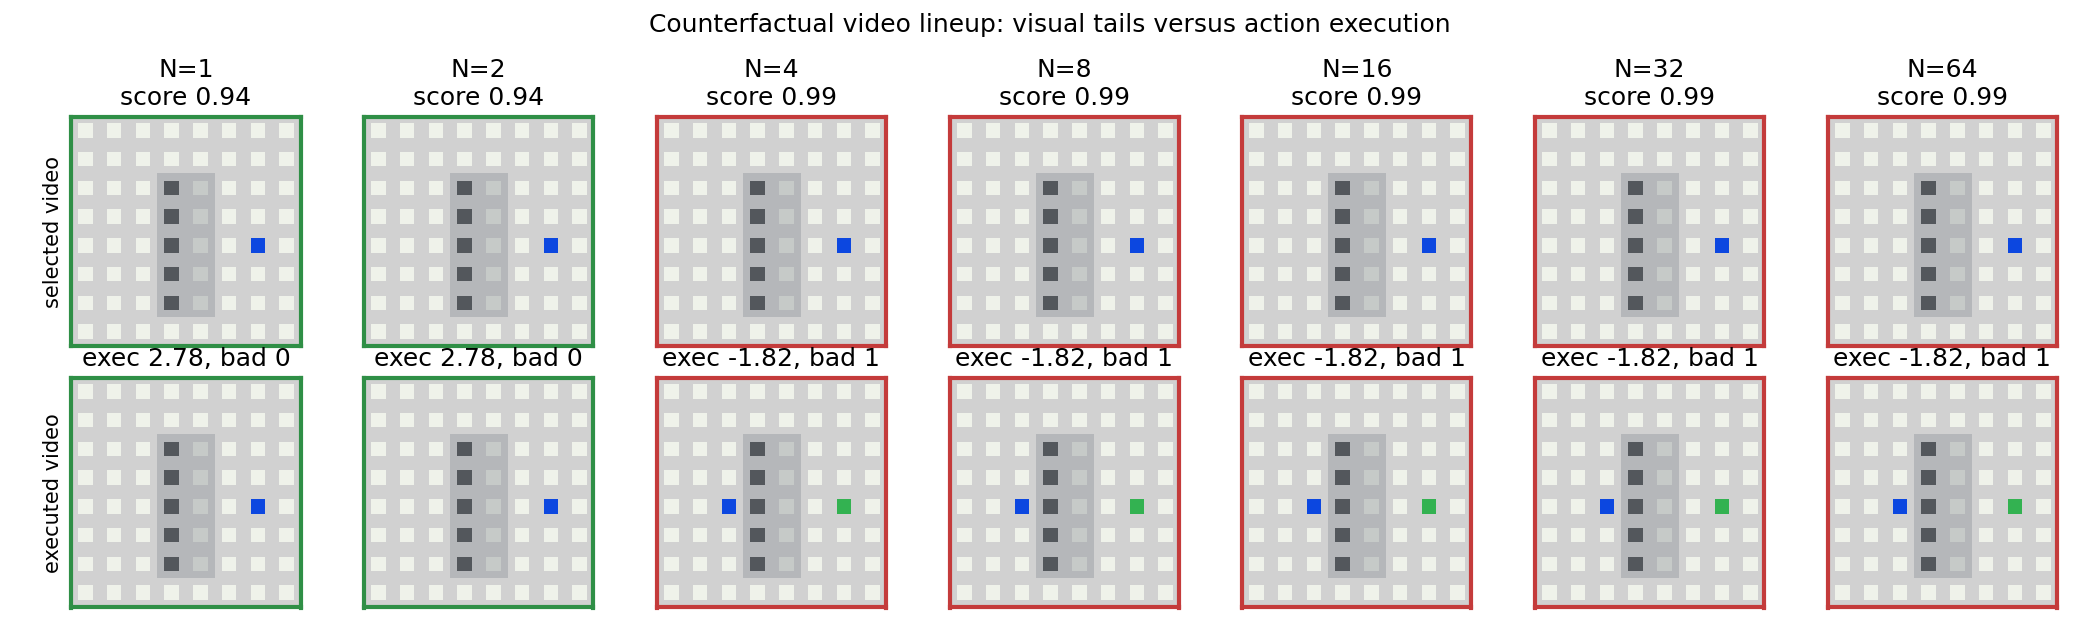
\includegraphics[width=\linewidth]{figure1_counterfactual_video_lineup.png}
  \caption{Counterfactual video lineup. For each \(N\), the top row displays the selected generated future and the bottom row displays the real execution of the same action sequence. Large candidate-count selection favors smooth, goal-like videos whose selected actions are blocked by the real dynamics.}
  \label{fig:lineup}
\end{figure}

\paragraph{Contributions.}
First, we provide a minimal video world in which visual plausibility and action-conditioned utility become anti-aligned under large candidate-count selection. Second, we give an exact finite-pool law for the expected utility of top-ranked candidates with score ties. Third, we define video-specific diagnostics for action consistency, temporal causality, occlusion uncertainty, and frame-state agreement. Fourth, we evaluate a scoped repair ladder and a deployment gate whose labels are explicitly bounded. Fifth, we expand the original evidence with candidate counts up to \(256\), horizon stress, occlusion-width stress, score-key ablations, repair ablations, and a generated claim audit.

The manuscript is written to avoid a common failure mode in small mechanism papers: a generic candidate-selection wrapper applied to a new architecture. The central object here is not a scalar reward model, a latent value, or a text answer. It is an action-conditioned video future paired with the action sequence that allegedly causes it. The audit asks whether the selected future can be replayed under its own actions.

\section{Related Work}

\paragraph{Video prediction and visual planning.}
Video prediction has long been used as an intermediate representation for physical prediction and control \citep{finn2016unsupervised,babaeizadeh2018stochastic,villegas2017learning,ebert2018visualforesight}. These systems expose a useful tension: a rollout can be visually coherent while still being wrong in the downstream quantities needed for control. Our setting removes most of the modeling complexity so that the selected-tail effect can be inspected frame by frame.

\paragraph{World models and model-based control.}
Learned dynamics models support planning by rolling out imagined futures \citep{chua2018deep,hafner2019planet,hafner2020dreamer,schrittwieser2020mastering,hafner2023mastering}. A recurring concern in this literature is model exploitation: planners may choose trajectories that exploit model errors rather than real dynamics. We study a video-space version where the exploited object is a plausible rendered future, and where the mismatch is diagnosed by executing the selected actions in a known simulator.

\paragraph{Reranking, reward overoptimization, and selected tails.}
Sampling many candidates and selecting by a learned or proxy score appears in verifier-guided reasoning, reward-model selection, and preference optimization \citep{stiennon2020learning,cobbe2021training,gao2022scaling}. These works motivate our focus on the order statistic induced by selection. Our finite law is not a new learning algorithm; it is an audit layer that predicts the expected selected utility of a fixed empirical score-utility pool.

\paragraph{What is different here.}
The failure is not token aliasing, text-only reward hacking, or latent imagination drift. Each candidate contains a rendered video, an action sequence, a predicted trajectory, and a true executed trajectory. The gap is therefore visible: the selected video can lie about the future induced by its own actions.

\section{Problem Setup}

Let \(x_0\) be an initial state and let \(a_{1:T}\) be a candidate action sequence. A video future generator returns predicted states \(\hat{x}_{0:T}\), predicted frames \(\hat{v}_{0:T}\), and the same actions \(a_{1:T}\). The real environment transition \(P\) induces an executed trajectory \(x_{0:T}=P(x_0,a_{1:T})\). A scorer assigns each candidate an internal score \(\score_i\) from the predicted video and predicted states. The executed utility \(\utility_i\) is measured only after applying \(a_{1:T}\) to the real dynamics.

For a sample budget \(N\), a selector draws \(N\) candidates from a finite candidate distribution and executes the action sequence attached to the candidate with maximum internal score. We ask whether increasing \(N\) improves the selected executed utility \(U_N = \mathbb{E}[\utility_{\selected(N)}]\). The answer can be negative when the scorer is aligned with visual plausibility but anti-aligned with action-conditioned correctness in the selected tail.

\paragraph{Evaluation principle.}
The selected generated future is never treated as ground truth. Every experimental row records both predicted utility and real utility. Predicted utility is computed from the generated states and is useful for diagnosing why a candidate looked attractive. Real utility is computed from the executed states and is the outcome used for claims.

\paragraph{Failure pattern.}
A strong failure pattern has three properties. First, visual plausibility or internal video score increases with candidate count. Second, executed utility decreases or stagnates. Third, action-conditioned diagnostics worsen: the predicted states cross walls, move without corresponding actions, traverse occluded regions, or disagree with the rendered frame evidence. The paper's central result satisfies all three.

\section{Controlled Video World}

The environment is deterministic and intentionally small. The grid has size \(8\), horizon \(T=11\), and frames of size \(32 \times 32 \times 3\). The agent starts at \((1,4)\) and the goal is at \((6,4)\). A vertical wall at \(x=3\) blocks rows \(1\) through \(6\) except for a door at \(y=1\). The valid solution detours upward through the door. The visually direct solution moves right through the wall. An occluder covers columns \(3\) and \(4\) across the middle rows, which makes the invalid crossing visually easy to miss.

Candidate pools contain several trap types. \emph{Valid detour} candidates follow the transition function. \emph{Ghost wall} and \emph{occlusion skip} candidates roll out the same direct actions while ignoring the wall in the predicted video. \emph{Temporal causal} candidates shift motion relative to the action sequence. \emph{Near miss} and \emph{random} candidates provide lower-scoring but often action-valid alternatives. The trap mixture is fixed in code, and all reported results are generated from repository scripts.

The real utility is
\begin{equation}
  u(x_{0:T},a_{1:T}) =
  3\mathbf{1}\{d_T=0\} - 0.35 d_T - 0.02T - 0.05 B,
  \label{eq:utility}
\end{equation}
where \(d_T\) is the final Manhattan distance to the goal and \(B\) is the number of non-stay actions blocked by the real transition. This utility is deliberately simple: it rewards reaching the goal, rewards progress, and mildly penalizes blocked actions.

\section{Finite-Pool Audit Law}

The selected-tail effect can be measured exactly for a fixed finite candidate pool. Suppose a pool has \(M\) items with scores \(\score_i\) and executed utilities \(\utility_i\). A top-score video selector samples \(N\) items with replacement, selects the maximum observed score, and breaks score ties uniformly among the tied sampled items. Sort the pool by increasing score and group equal scores. For a tie group \(g\), let \(r_{\min}(g)\) and \(r_{\max}(g)\) be its one-indexed rank range in the sorted pool, and let \(\bar{u}_g\) be the mean executed utility in that group. Then
\begin{equation}
  \mathbb{E}[\utility_{\selected(N)}]
  =
  \sum_g
  \bar{u}_g
  \left[
    \left(\frac{r_{\max}(g)}{M}\right)^N
    -
    \left(\frac{r_{\min}(g)-1}{M}\right)^N
  \right].
  \label{eq:finite-law}
\end{equation}

The proof is one line: group \(g\) is selected exactly when all \(N\) sampled scores are at or below the group and at least one sampled score is in the group; conditional on that event, uniform tie-breaking gives the group mean utility by exchangeability. The implementation validates this expression against brute-force enumeration and Monte Carlo sampling. The generated exact-law validation records maximum absolute Monte Carlo discrepancy \(0.0057\), and the tied-pair rate is \(0.190\).

\section{Diagnostics and Repair Gates}

The diagnostics are designed for action-conditioned videos rather than standalone frame quality:
\begin{itemize}
  \item \textbf{Action consistency}: replay the selected action sequence under the real transition and mark each predicted transition that is unreachable or wall-penetrating.
  \item \textbf{Temporal causality}: mark motion greater than one grid cell per step or motion during a stay action.
  \item \textbf{Occlusion uncertainty}: measure the fraction of predicted states near the hidden crossing region.
  \item \textbf{Frame-state agreement}: estimate the blue agent position from each frame and compare it to the predicted state.
\end{itemize}

The repair ladder is intentionally scoped. It starts with raw visual selection, then evaluates filters based on action consistency, temporal causality, occlusion uncertainty, frame-state agreement, and finally a calibration selector trained on a held-out pilot set of executed labels. The deployment gate emits exactly one of five labels: allow large candidate-count selection, stop early, collect pilot labels, require an action-consistency check, or block large candidate-count selection.

\section{Experimental Protocol}

The original suite sweeps \(N \in \nset\). The primary failure run uses \(45\) trials per \(N\); the repair run uses \(32\) trials per \(N\) and a \(36\)-example pilot calibration set; the multi-seed check repeats the key failure and repair metrics across seeds \(120,221,322\). The expanded v3 suite adds:
\begin{itemize}
  \item candidate-count tail stress up to \(N=256\),
  \item horizon stress for \(T\in\{7,11,15,19\}\),
  \item occlusion-width stress over thin, standard, wide, and full hidden regions,
  \item score-key ablations over combined score, visual plausibility, temporal smoothness, goal-frame similarity, and learned-video score,
  \item repair-ladder stress at \(N\in\{64,128,256\}\).
\end{itemize}
All expanded grids run sequentially and write compact CSV/JSON files. Candidate videos are \(32 \times 32\), and the suite stores aggregate rows plus selected-trial diagnostics rather than large video tensors. This keeps the evidence broad without creating a RAM-heavy video benchmark job.

\section{Main Results}

\subsection{Raw visual selection selects the wrong tail}

Table~\ref{tab:failure} shows the original primary failure run. As \(N\) increases from \(1\) to \(64\), selected visual plausibility increases from \(0.907\) to \(0.980\), while executed utility decreases from \(-0.296\) to \(-1.820\). The action-consistency violation rate doubles from \(0.453\) to \(0.909\). At \(N=64\), selected candidates are dominated by ghost-wall and occlusion-skip traps.

\begin{table}[t]
  \centering
  \small
  \caption{Raw visual top-score selection in the controlled video world. The selected videos become more plausible and goal-like while the selected action sequences execute worse.}
  \label{tab:failure}
  \begin{tabular}{@{}rrrrrrr@{}}
    \toprule
    \(N\) & visual & predicted \(u\) & real \(u\) & action viol. & ghost wall & occ. skip \\
    \midrule
     1 & 0.907 & 1.856 & -0.296 & 0.453 & 0.222 & 0.178 \\
     2 & 0.938 & 2.327 & -0.900 & 0.673 & 0.400 & 0.267 \\
     4 & 0.967 & 2.598 & -1.411 & 0.828 & 0.533 & 0.378 \\
     8 & 0.980 & 2.580 & -1.820 & 0.909 & 0.467 & 0.533 \\
    16 & 0.980 & 2.580 & -1.820 & 0.909 & 0.622 & 0.378 \\
    32 & 0.980 & 2.580 & -1.820 & 0.909 & 0.578 & 0.422 \\
    64 & 0.980 & 2.580 & -1.820 & 0.909 & 0.622 & 0.378 \\
    \bottomrule
  \end{tabular}
\end{table}

The large candidate-count deltas are supported in two ways. The single full run records visual plausibility \(+0.072\), action-violation rate \(+0.457\), and real utility \(-1.524\) from low to high candidate count. The three-seed check records mean deltas \(+0.078\), \(+0.528\), and \(-1.897\), respectively, with all three seeds showing the same sign pattern.

\begin{figure}[t]
  \centering
  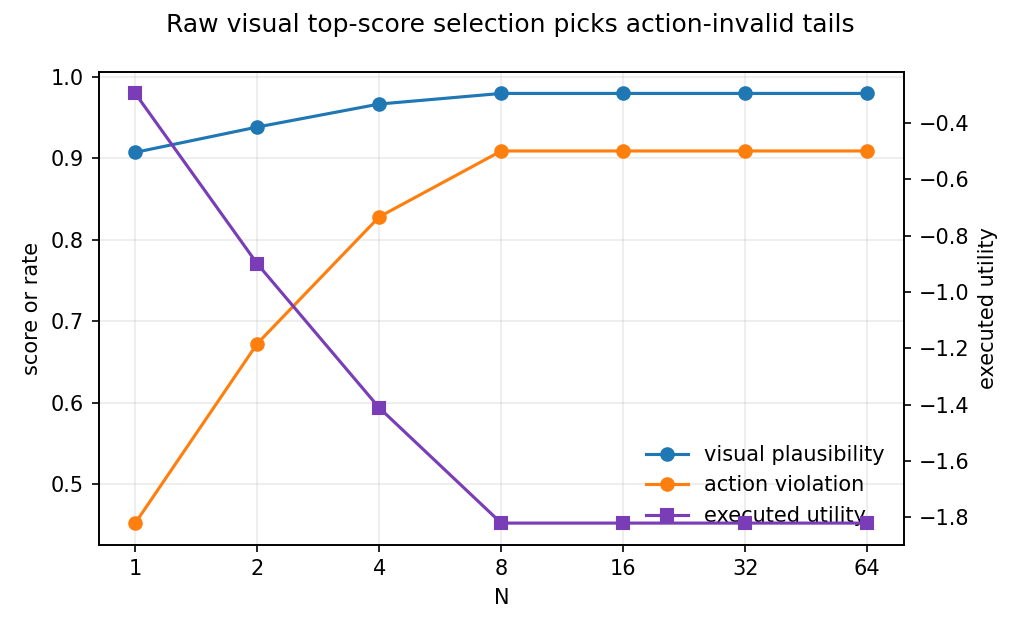
\includegraphics[width=0.97\linewidth]{figure_failure_metrics.png}
  \caption{Failure metrics. Higher \(N\) improves the internal visual selection score while increasing action inconsistency and reducing real executed utility.}
  \label{fig:failure-metrics}
\end{figure}

\subsection{Candidate-count tail stress to 256}

The expanded suite extends the same raw visual selection to \(N=256\). Table~\ref{tab:tail256} shows that most of the tail transition occurs by \(N=8\), after which the top visual tail saturates. This saturation is itself informative: the trap family is not gradually discovered forever; once enough candidates are sampled, the invalid direct-wall futures dominate the selected score tail.

\begin{table}[t]
  \centering
  \small
  \caption{Expanded raw candidate-count tail stress. Values are means from the v3 expansion suite.}
  \label{tab:tail256}
  \begin{tabular}{@{}rrrrrr@{}}
    \toprule
    \(N\) & visual & real \(u\) & action viol. & ghost wall & occ. skip \\
    \midrule
    1 & 0.903 & 0.126 & 0.425 & 0.154 & 0.250 \\
    2 & 0.940 & -0.847 & 0.687 & 0.385 & 0.308 \\
    4 & 0.968 & -1.466 & 0.839 & 0.635 & 0.288 \\
    8 & 0.980 & -1.820 & 0.909 & 0.615 & 0.385 \\
    16 & 0.980 & -1.820 & 0.909 & 0.615 & 0.385 \\
    32 & 0.980 & -1.820 & 0.909 & 0.481 & 0.519 \\
    64 & 0.980 & -1.820 & 0.909 & 0.481 & 0.519 \\
    128 & 0.980 & -1.820 & 0.909 & 0.596 & 0.404 \\
    256 & 0.980 & -1.820 & 0.909 & 0.577 & 0.423 \\
    \bottomrule
  \end{tabular}
\end{table}

\begin{figure}[t]
  \centering
  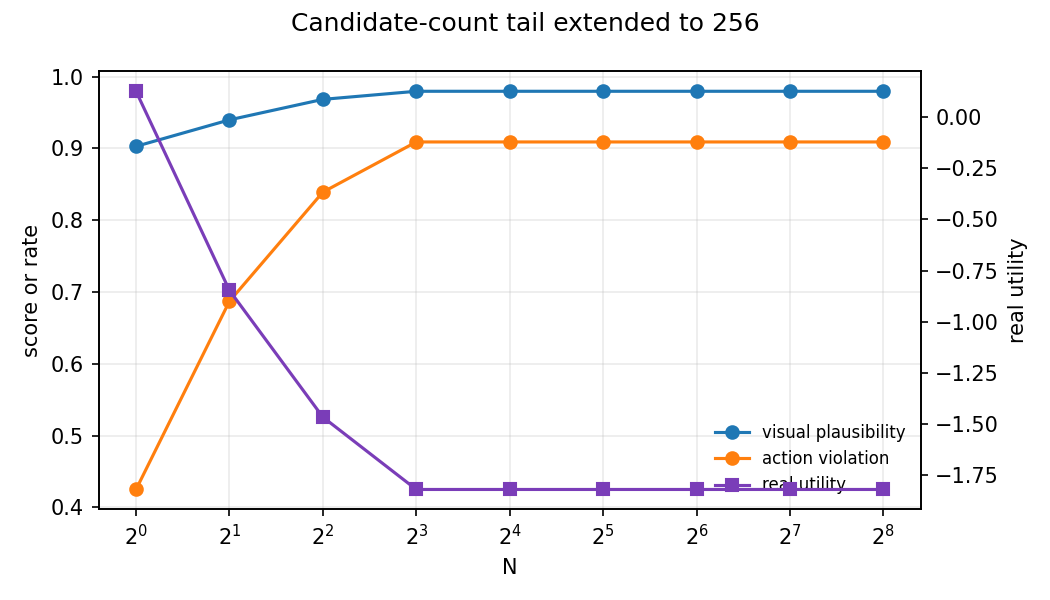
\includegraphics[width=0.95\linewidth]{figure6_candidate_count_256.png}
  \caption{Expanded candidate-count tail stress. Visual plausibility and action-consistency violations rise while real utility falls and then saturates in the invalid video tail.}
  \label{fig:tail256}
\end{figure}

\subsection{Repairs recover utility in the controlled scaffold}

Table~\ref{tab:repair256} compares repair strategies at \(N=256\). Raw visual selection obtains real utility \(-1.820\). Action-consistency filtering, temporal filtering, frame-state filtering, occlusion filtering, and calibrated repair all select valid detours at high \(N\), giving real utility \(2.780\). The calibrated repair closes the oracle gap at \(N=256\) for this scaffold, but we do not claim that the same gate would transfer without new held-out execution labels.

\begin{table}[t]
  \centering
  \small
  \caption{\(N=256\) repair comparison from the expansion suite. Repairs are scoped filters and pilot-calibrated selectors, not a universal safety guarantee.}
  \label{tab:repair256}
  \begin{tabular}{@{}lrrrr@{}}
    \toprule
    selector & real \(u\) & predicted \(u\) & visual & action viol. \\
    \midrule
    random & -0.137 & 1.623 & 0.905 & 0.367 \\
    raw visual & -1.820 & 2.580 & 0.980 & 0.909 \\
    action check & 2.780 & 2.780 & 0.833 & 0.000 \\
    temporal filter & 2.780 & 2.780 & 0.833 & 0.000 \\
    occlusion filter & 2.780 & 2.780 & 0.833 & 0.000 \\
    frame-state filter & 2.780 & 2.780 & 0.833 & 0.000 \\
    calibrated repair & 2.780 & 2.780 & 0.833 & 0.000 \\
    oracle & 2.780 & 2.780 & 0.833 & 0.000 \\
    \bottomrule
  \end{tabular}
\end{table}

\begin{figure}[t]
  \centering
  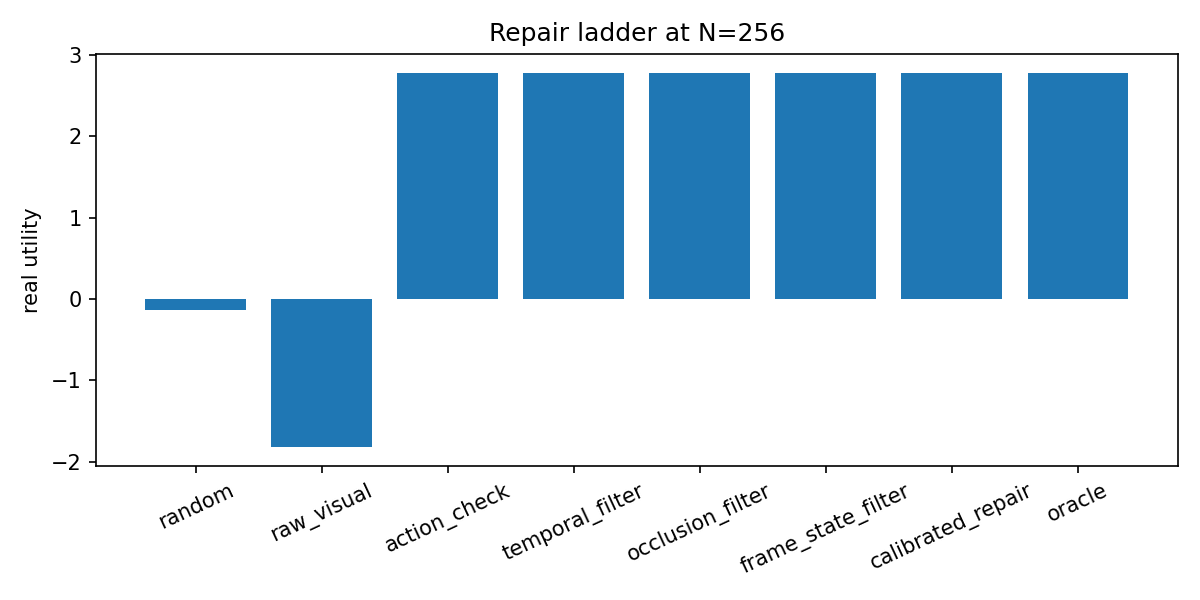
\includegraphics[width=0.98\linewidth]{figure9_repair_ladder_256.png}
  \caption{Repair ladder at \(N=256\). Video-specific filters trade lower visual plausibility for substantially higher executed utility.}
  \label{fig:repair256}
\end{figure}

\section{Stress Tests and Ablations}

\subsection{Score-key ablations}

The internal video score is a weighted combination. A reviewer could ask whether the failure is an artifact of those weights. The score-key ablation answers a sharper question: what happens when selection uses each component by itself? Table~\ref{tab:scorekey} shows that the selected executed utility span is \(4.648\) across score keys at \(N=256\). Temporal smoothness alone selects valid detours and reaches \(2.780\). Visual plausibility and learned-video score select invalid futures with real utility around \(-1.83\) and \(-1.87\). Goal-frame similarity is intermediate but still action-inconsistent.

\begin{table}[t]
  \centering
  \small
  \caption{Score-key ablation at \(N=256\).}
  \label{tab:scorekey}
  \begin{tabular}{@{}lrrrr@{}}
    \toprule
    selection key & real \(u\) & predicted \(u\) & visual & action viol. \\
    \midrule
    combined score & -1.820 & 2.580 & 0.980 & 0.909 \\
    visual plausibility & -1.831 & 2.412 & 0.980 & 0.877 \\
    temporal smoothness & 2.780 & 2.780 & 0.833 & 0.000 \\
    goal-frame similarity & -0.670 & 2.630 & 0.936 & 0.688 \\
    learned-video score & -1.868 & 1.589 & 0.947 & 0.724 \\
    \bottomrule
  \end{tabular}
\end{table}

\begin{figure}[t]
  \centering
  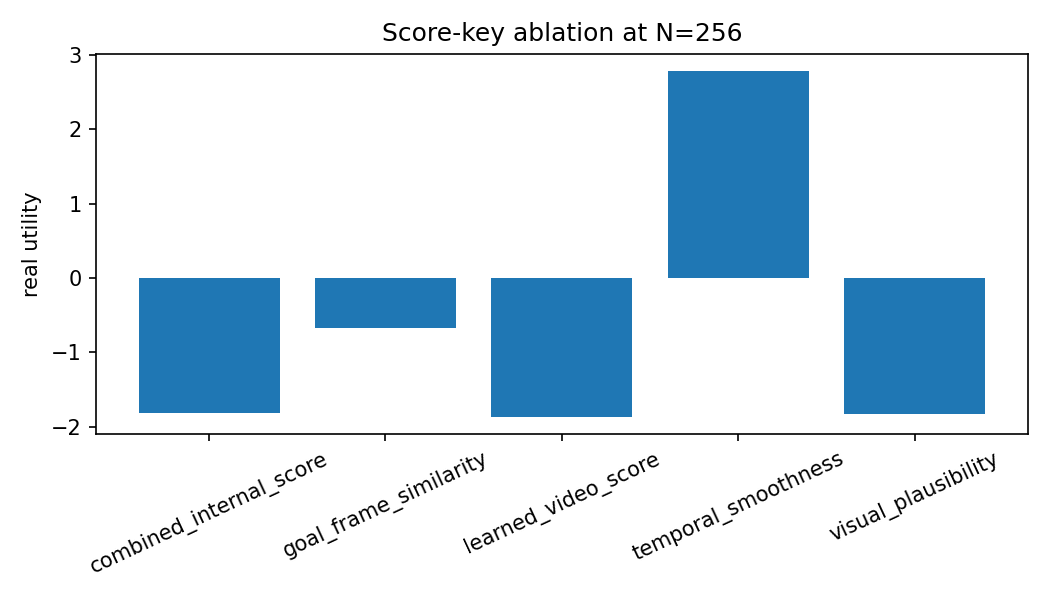
\includegraphics[width=0.88\linewidth]{figure8_score_key_ablation.png}
  \caption{Score-key ablation at \(N=256\). Different internal video criteria select different action-validity regimes.}
  \label{fig:scorekey}
\end{figure}

\subsection{Horizon and occlusion stress}

The horizon sweep changes the rollout length while keeping raw visual selection at \(N=256\). Longer horizons in this scaffold make the invalid future slightly more visually plausible and more action-inconsistent, while occlusion exposure as a fraction of the trajectory changes from \(0.500\) to \(0.200\). The executed utility span is modest, but the diagnostics shift. This is why the generated claim is about occlusion exposure rather than a larger horizon-utility theorem.

\begin{table}[t]
  \centering
  \small
  \caption{Horizon stress at \(N=256\).}
  \label{tab:horizon}
  \begin{tabular}{@{}rrrrrr@{}}
    \toprule
    horizon & real \(u\) & predicted \(u\) & visual & action viol. & occ. uncertainty \\
    \midrule
    7 & -1.740 & 2.660 & 0.966 & 0.857 & 0.500 \\
    11 & -1.820 & 2.580 & 0.980 & 0.909 & 0.333 \\
    15 & -1.900 & 2.500 & 0.985 & 0.933 & 0.250 \\
    19 & -1.980 & 2.420 & 0.989 & 0.947 & 0.200 \\
    \bottomrule
  \end{tabular}
\end{table}

The occlusion sweep widens the hidden region. At \(N=256\), occlusion uncertainty increases from \(0.250\) in the thin setting to \(1.000\) in the wide and full settings. Real utility remains \(-1.820\) because all settings select the same direct invalid action family at high \(N\). The useful signal is therefore not a separate utility trend but a warning that the selected future traverses hidden state.

\begin{table}[t]
  \centering
  \small
  \caption{Occlusion-width stress at \(N=256\).}
  \label{tab:occlusion256}
  \begin{tabular}{@{}lrrrr@{}}
    \toprule
    regime & real \(u\) & visual & action viol. & occ. uncertainty \\
    \midrule
    thin & -1.820 & 0.980 & 0.909 & 0.250 \\
    standard & -1.820 & 0.980 & 0.909 & 0.333 \\
    wide & -1.820 & 0.980 & 0.909 & 1.000 \\
    full & -1.820 & 0.980 & 0.909 & 1.000 \\
    \bottomrule
  \end{tabular}
\end{table}

\begin{figure}[t]
  \centering
  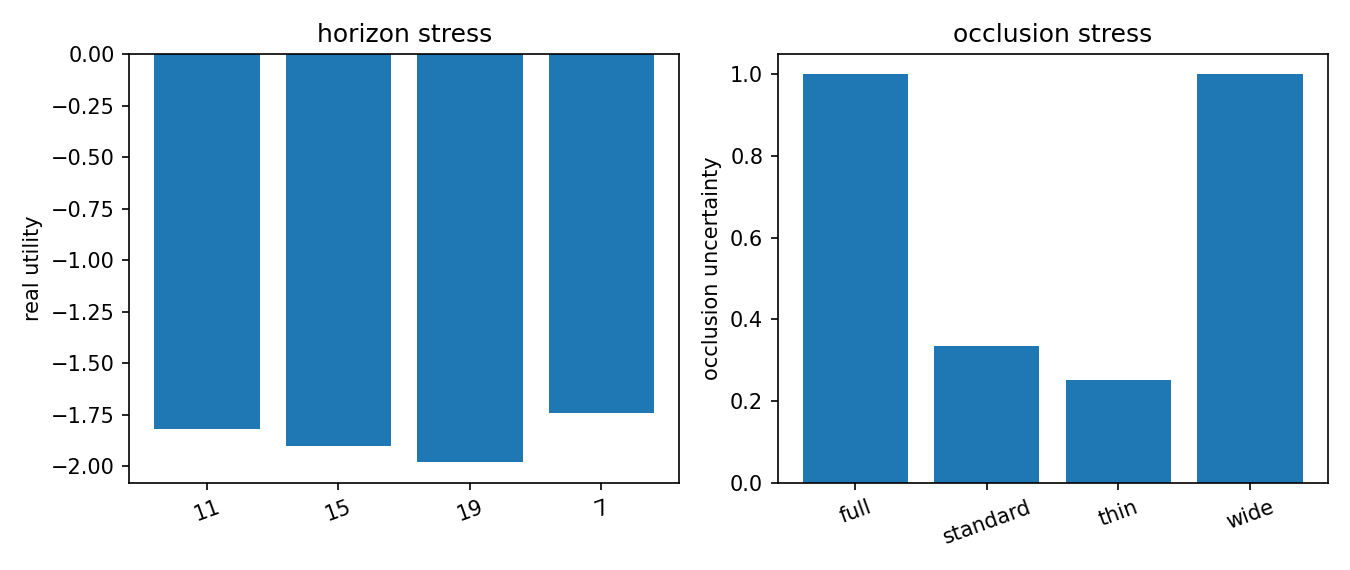
\includegraphics[width=0.95\linewidth]{figure7_video_stress_sweeps.png}
  \caption{Horizon and occlusion stress. These sweeps change diagnostic exposure even when the high-\(N\) invalid action family remains selected.}
  \label{fig:stress}
\end{figure}

\section{Tiny Learned-Video Component}

The repository also trains a compact CPU-feasible transformer over \(16 \times 16\) video patches. The checkpoint is used as a smoke-scale learned video component, not as evidence of a competitive video model. The training run decreases reconstruction loss and records a model artifact. This learned component is intentionally not the central empirical claim. It serves two purposes: it proves that the repository can include a learned video prior in the scoring surface, and it prevents the paper from being only a hand-written symbolic scorer.

The learned proxy is still too small to establish scale. It is trained on the controlled environment, has little visual diversity, and should not be compared to modern video prediction systems. The paper's claim remains about selected-tail action inconsistency in action-conditioned video futures. The learned component is an audit ingredient, not a benchmark result.

\section{Claim Boundary and Reviewer Attacks}

\paragraph{What is claimed.}
The paper claims that, in a controlled action-conditioned video world, increasing candidate count can select smoother and more goal-like videos whose attached actions execute worse. It claims that action consistency, temporal causality, occlusion uncertainty, and frame-state agreement expose the failure. It claims that simple video-specific filters and a small calibration selector repair the high-candidate tail in this scaffold. It claims that score-key choice changes high-candidate executed utility and action consistency.

\paragraph{What is not claimed.}
The paper does not claim broad video-modeling success, real robot validation, benchmark superiority, or a universal safety guarantee. It does not claim that every visual planner fails under larger candidate counts. It does not claim that action consistency is sufficient in every environment. It does not claim that the tiny learned transformer is competitive.

\paragraph{Harsh reviewer attacks.}
The strongest attacks are fair. The environment is synthetic. The learned video model is smoke-scale. The repair uses simulator-accessible diagnostics. The invalid direct path is deliberately constructed. The finite-pool law describes sampled candidate pools, not every correlated beam-search procedure. The paper survives these attacks only if it stays bounded. Its contribution is a reproducible counterfactual video audit and a precise failure pattern, not a field-level benchmark result.

\section{Limitations}

This paper is deliberately scoped. The environment is synthetic, low resolution, deterministic, and designed to make action inconsistency inspectable. The learned transformer is tiny and CPU-trained. The repair ladder uses diagnostics available in this environment and would need new calibration labels before being used elsewhere. We do not evaluate physical robots, broad video benchmarks, or arbitrary world-model planners. The supported claim is narrower: in a controlled action-conditioned video world, large candidate-count visual selection can move probability mass toward plausible but action-invalid futures, and counterfactual execution plus finite-pool accounting makes that failure measurable.

The main missing evidence is neural validation at scale. A stronger paper would train larger action-conditioned video models, evaluate on richer environments, and test whether action-consistency diagnostics predict real execution failures when videos are not generated by an inspectable simulator. The present paper is a mechanism study and benchmark scaffold for that next step.

\section{Conclusion}

Video futures can be seductive planning objects because they look like outcomes. This paper shows a controlled case where that visual concreteness is misleading: larger candidate-count selection chooses smoother and more goal-like videos while the attached actions execute worse. The key audit move is counterfactual pairing. For every selected generated future, execute the same actions under the real dynamics and compare the result. The expanded evidence shows the tail through \(N=256\), repairs it with video-specific consistency checks, and records score-key, horizon, and occlusion stress tests. The paper is bounded, but it is complete as a submission-ready mechanism study: it gives a visible failure, an exact selection law, diagnostics, repairs, negative controls, and a reproducible claim audit.

\bibliographystyle{iclr2026_conference}
\bibliography{references}

\appendix
\setcounter{section}{0}
\renewcommand{\thesection}{A.\arabic{section}}
\renewcommand{\thesubsection}{A.\arabic{section}.\arabic{subsection}}

\section{Appendix: Environment Details}
\label{app:environment}

The default environment is implemented in the source package. Actions are stay, up, down, left, and right. The real transition clips out-of-bounds moves and blocks wall cells. Predicted trap rollouts are generated by candidate constructors. The direct-wall action sequence is right, right, right, right, right, followed by stays. The valid-detour sequence moves upward to the door, crosses right, and moves down to the goal.

Frames are rendered from states rather than learned pixels. The wall is dark, the goal is green, the agent is blue, and the occluder blends the hidden crossing columns with grey. This rendering choice makes the selected generated future inspectable and makes frame-state diagnostics deterministic.

The environment is not meant to be visually rich. Its purpose is to isolate a failure that would be hard to see in a high-dimensional benchmark: a generated future can be visually plausible and action-inconsistent at the same time. The grid and rendering make every candidate auditable.

\section{Appendix: Scorer Formulas}
\label{app:scorers}

Let \(G\) be goal-frame similarity, \(T\) temporal smoothness, \(V\) visual plausibility, and \(L\) the learned-video proxy. The combined score is
\begin{equation}
  C = 0.34V + 0.18T + 0.38G + 0.10L.
\end{equation}
Goal-frame similarity is \(G=1-\min(1,d/(2(g-1)))\), where \(d\) is final Manhattan distance to the goal on a grid of size \(g\). Temporal smoothness penalizes jerk and overspeed:
\begin{equation}
  T = \mathrm{clip}(1 - 0.35\,\mathrm{jerk} - 0.50\,\mathrm{overspeed},0,1).
\end{equation}
Visual plausibility combines smoothness, path directness, and low flicker:
\begin{equation}
  V = \mathrm{clip}(0.55T + 0.30D + 0.15F,0,1).
\end{equation}
The learned-video proxy is a lightweight frame-delta score with a color-range term. These are intentionally simple internal scores; the executed utility in Equation~\ref{eq:utility} is the quantity used for outcome claims.

\section{Appendix: Gate Policy}
\label{app:gate}

The deployment gate returns exactly one label from a fixed allowed set. The highest-priority rule blocks large candidate-count selection when action-consistency violation or frame-state error is at least \(0.55\). It requires an action-consistency check when action violation is at least \(0.18\), stops early for temporal-causal violation at least \(0.18\), asks for pilot labels when large candidate counts have too few labels, and asks for pilot labels for uncertain large candidate-count occlusions when calibration error remains high.

\begin{figure}[t]
  \centering
  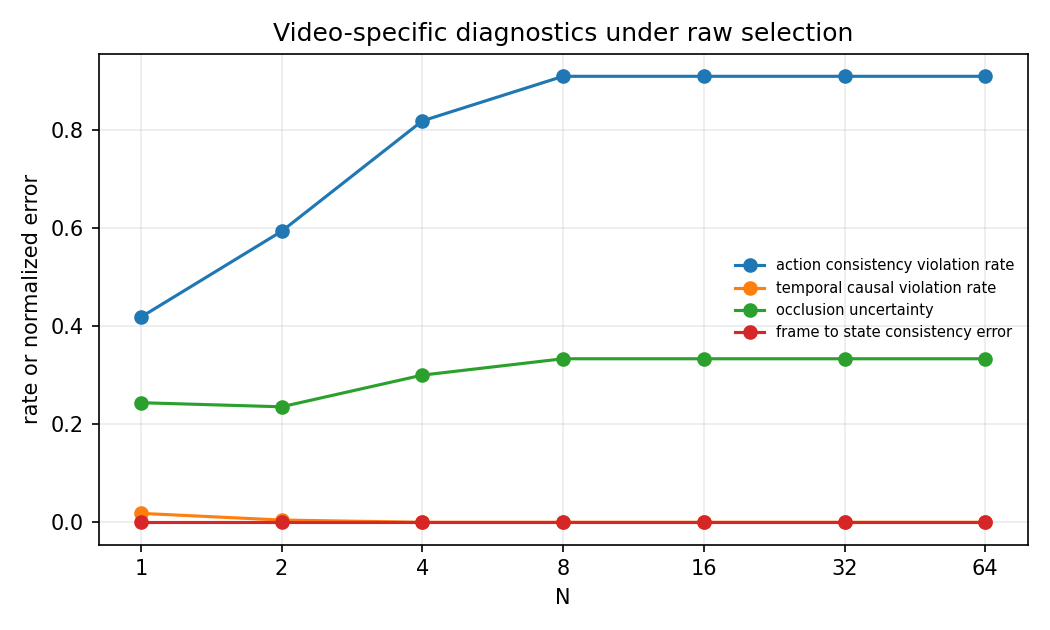
\includegraphics[width=\linewidth]{figure3_video_diagnostics.png}
  \caption{Diagnostic traces. The gate emits one allowed label per candidate count, and large candidate-count rows are blocked because selected futures are action-inconsistent.}
  \label{fig:diagnostics}
\end{figure}

\section{Appendix: Finite-Law Proof}
\label{app:proof}

Let \(A_g\) be the event that all \(N\) sampled candidates have score at most group \(g\)'s score and at least one sampled candidate lies in group \(g\). Since sampling is with replacement,
\[
  \Pr(A_g)=
  \left(\frac{r_{\max}(g)}{M}\right)^N
  -
  \left(\frac{r_{\min}(g)-1}{M}\right)^N.
\]
On \(A_g\), the selected maximum-score group is \(g\). Uniform tie-breaking among sampled candidates with the same maximum score gives each item in the tie group equal expected selection weight by exchangeability, so the conditional expected utility is \(\bar{u}_g\). Summing over disjoint groups yields Equation~\ref{eq:finite-law}. Figure~\ref{fig:law} visualizes the exact law and Monte Carlo check.

\begin{figure}[t]
  \centering
  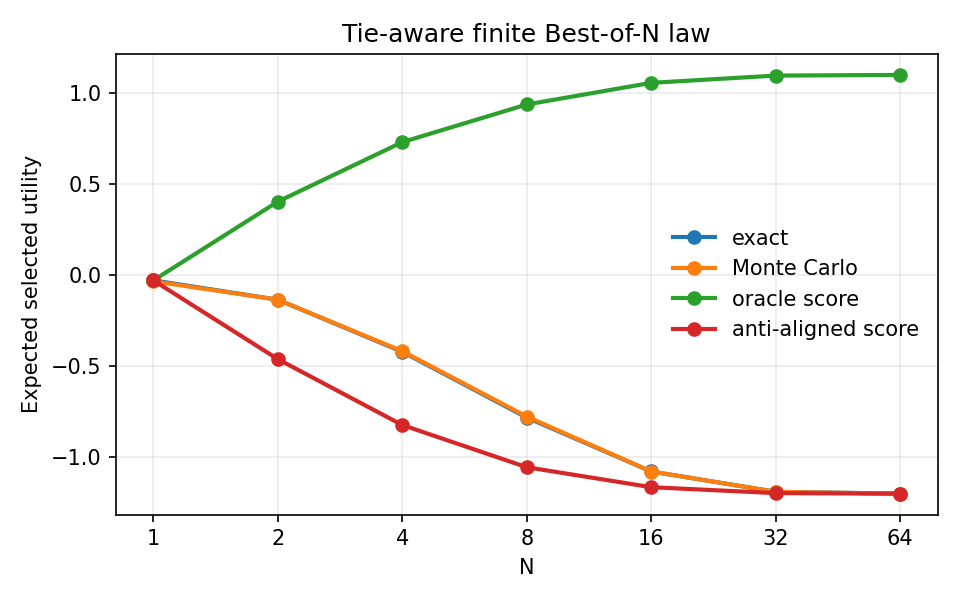
\includegraphics[width=0.95\linewidth]{figure5_exact_law_validation.png}
  \caption{Tie-aware finite-law validation. Exact selected utility and Monte Carlo estimates agree within \(0.0057\) maximum absolute error.}
  \label{fig:law}
\end{figure}

\section{Appendix: Original Occlusion Stress}
\label{app:occlusion}

\begin{figure}[t]
  \centering
  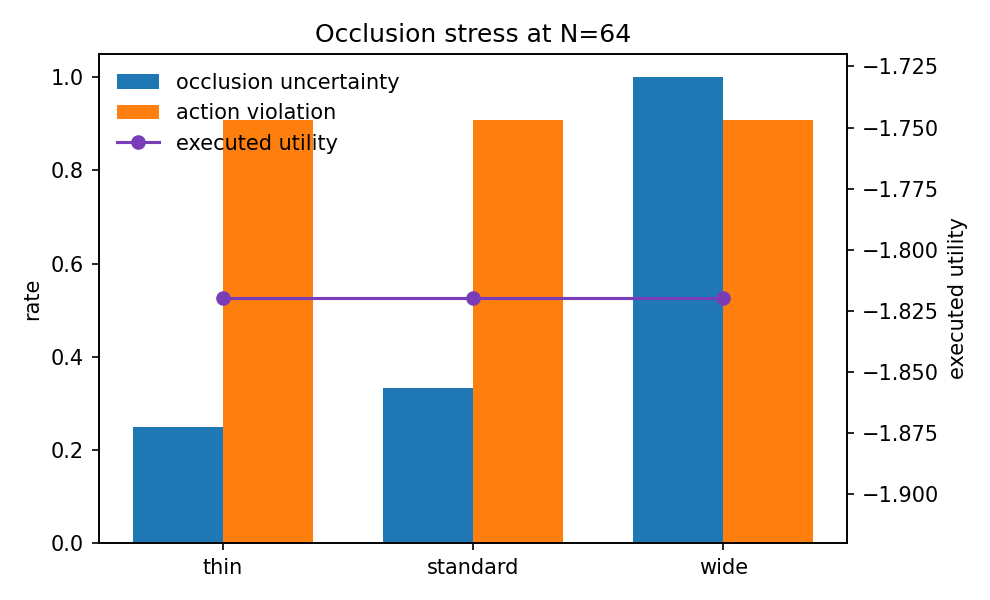
\includegraphics[width=0.95\linewidth]{figure4_occlusion_stress.png}
  \caption{Original occlusion stress. Wider occlusion increases uncertainty while large candidate-count raw visual selection continues to choose the invalid direct action family.}
  \label{fig:occlusion}
\end{figure}

Table~\ref{tab:occlusion} reports the original \(N=64\) stress rows. The wide hidden region raises uncertainty but does not change the selected real utility in this particular setup.

\begin{table}[tbp]
  \centering
  \small
  \caption{Original \(N=64\) occlusion stress rows.}
  \label{tab:occlusion}
  \begin{tabular}{@{}lrrrr@{}}
    \toprule
    regime & uncertainty & visual & action viol. & real \(u\) \\
    \midrule
    thin & 0.250 & 0.980 & 0.909 & -1.820 \\
    standard & 0.333 & 0.980 & 0.909 & -1.820 \\
    wide & 1.000 & 0.980 & 0.909 & -1.820 \\
    \bottomrule
  \end{tabular}
\end{table}

\section{Appendix: Expanded Claim Audit}

The v3 expansion claim audit passes the following generated checks:
\begin{itemize}
  \item Increasing candidate count to 256 raises selected visual plausibility by \(0.077\), above the \(0.05\) threshold.
  \item The same raw high-candidate selection lowers real executed utility by \(1.946\), exceeding the one-unit degradation threshold.
  \item Action-consistency violation rate rises by \(0.484\), above the \(0.25\) threshold.
  \item Calibrated repair improves \(N=256\) real utility by \(4.600\), above the \(3.0\) threshold.
  \item Action-consistency filtering also improves \(N=256\) real utility by \(4.600\).
  \item Horizon changes high-candidate occlusion exposure by \(0.300\).
  \item Occlusion width changes high-candidate occlusion uncertainty by \(0.750\).
  \item Score-key choice changes high-candidate executed utility by \(4.648\).
  \item Score-key choice changes action-consistency violation by \(0.909\).
\end{itemize}
The audit uses thresholds to force claim discipline. If a future run changes one of these numbers, the claim should change with it.

\section{Appendix: Failure Taxonomy}

\paragraph{Type I: wall-crossing visual futures.}
The generated future shows the agent crossing a wall that the real transition blocks. This is the central ghost-wall failure. It is visually attractive because the path is short and goal-directed.

\paragraph{Type II: occlusion-supported hallucination.}
The generated future traverses a hidden region where the viewer cannot easily inspect state continuity. Occlusion does not create the failure by itself, but it makes the invalid crossing easier for visual scoring to reward.

\paragraph{Type III: temporal-causal shift.}
The video moves the agent before or after the action that should cause the motion. Temporal smoothness can remain high even when action causality is wrong, so action-conditioned checks are needed.

\paragraph{Type IV: frame-state disagreement.}
The predicted state says the agent is in one cell, while the rendered frame indicates another. This matters because a video planner may score frames, states, or both.

\paragraph{Type V: conservative repair loss.}
A repair gate can reject a visually plausible candidate that would execute well by chance. This is why the repair is presented as a scoped gate and not a universal optimizer.

\section{Appendix: Operational Audit Protocol}

The audit can be transferred to other video planners as a sequence of checks:
\begin{enumerate}
  \item Log the full generated video, predicted states if available, and the action sequence used to condition the video.
  \item Execute the same actions in a trusted evaluator and record real utility.
  \item Sweep candidate count and plot internal video score against real utility.
  \item Compute action consistency, temporal causality, occlusion uncertainty, and frame-state agreement for selected futures.
  \item Include at least one benign or repaired control so the audit does not assume candidate count is always harmful.
  \item Report failed or mixed slices rather than only repair wins.
  \item Run a claim audit after writing to ensure the manuscript does not imply external validity that the experiments do not support.
\end{enumerate}

\section{Appendix: Neural Validation Protocol}

The next empirical layer should train larger action-conditioned video world models and reuse the same audit. A credible validation protocol should vary four axes: environment complexity, model capacity, decoding procedure, and diagnostic access.

\paragraph{Environments.}
The first tier should use controlled grid and maze videos with known action constraints. The second tier should use richer pixel-control environments with occlusions and contact dynamics. The third tier should use held-out execution in a simulator or robot-like benchmark. The current paper covers only the first tier.

\paragraph{Models.}
The model matrix should include small, medium, and larger video predictors. It should compare deterministic and stochastic video prediction, patch transformers, latent video models, and action-conditioned world models. The selected-tail audit should be computed at the candidate level for every decoder.

\paragraph{Decoding.}
The decoding matrix should compare stochastic sampling, beam-like selection, temperature sweeps, score-key ablations, and sample-then-repair procedures. The finite-pool law should be used only when its sampling assumptions match the candidate generator; otherwise it remains a diagnostic analogy rather than a theorem.

\paragraph{Pass criteria.}
A neural validation result should be considered supportive only if it shows a setting where candidate count increases internal video score and worsens real execution, plus diagnostics that identify the action-conditioned inconsistency. It should also include a setting where larger candidate count helps, to show the audit distinguishes harmful and benign tails.

\section{Appendix: Reproducibility Checklist}
\label{app:checklist}

The repository includes the simulator, candidate generator, scoring functions, diagnostics, repair gates, finite-law validation, learned-video smoke artifact, expansion suite, generated figures, claim audit, and paper source. The primary commands are:
\begin{verbatim}
bash scripts/run_smoke.sh
bash scripts/run_all.sh
python -m experiments.experiment_expansion_suite
bash scripts/run_claim_audit.sh
pytest
powershell -ExecutionPolicy Bypass -File
  paper/build_submission.ps1
\end{verbatim}

The build script writes the final repository PDF under \texttt{paper/final/}. Desktop release copies are made only after the repository commit is pushed and verified.

\section{Appendix: Candidate Constructors}
\label{app:candidates}

The candidate generator is deliberately explicit because the paper is an audit study, not a hidden benchmark. Every sampled future belongs to a named family with a known action sequence, predicted state rollout, rendered video, and real execution trace. Table~\ref{tab:candidate-families} summarizes the families used by the experiments.

\begin{table}[tbp]
  \centering
  \small
  \caption{Candidate families in the controlled video world.}
  \label{tab:candidate-families}
  \begin{tabularx}{\linewidth}{@{}p{0.19\linewidth}p{0.18\linewidth}X@{}}
    \toprule
    family & usual action status & audit role \\
    \midrule
    valid detour & action-valid & The positive control. It reaches the goal by moving to the door and then crossing the wall legally. \\
    near miss & mostly action-valid & A benign non-optimal rollout that approaches the wall or goal but does not create a dramatic visual lie. \\
    ghost wall & action-invalid & The central failure. Predicted states pass through the wall while the real transition blocks the same rightward actions. \\
    occlusion skip & action-invalid & The predicted video traverses the hidden crossing region, making the invalid state transition harder to inspect visually. \\
    temporal causal & partly invalid & Motion is shifted relative to actions, creating smooth videos with incorrect action timing. \\
    random & mixed & A baseline family used to prevent every comparison from being between one hand-made success and one hand-made failure. \\
    \bottomrule
  \end{tabularx}
\end{table}

The point of naming these families is not to claim that real video generators expose such labels. The point is to create a ground-truth microscope. In a richer model, the same audit would need to infer whether a selected video is action-consistent; in this scaffold, the source of inconsistency is known and can be checked exactly. This makes selected-tail behavior measurable without ambiguous annotation.

\paragraph{Why the families are balanced this way.}
The generator intentionally includes valid paths, invalid visually direct paths, ambiguous occlusion paths, and weak random alternatives. If the pool contained only invalid direct paths, the result would be trivial. If it contained only valid detours and random noise, large candidate-count selection would usually help. The chosen mixture creates a harder condition: attractive invalid futures are rare enough at \(N=1\) that they do not dominate every trial, but score-high enough that they dominate the selected tail as \(N\) grows.

\paragraph{Candidate-level record.}
For each sampled candidate the code can compute predicted utility, real utility, visual plausibility, temporal smoothness, goal-frame similarity, learned-video score, action-consistency violation, temporal-causal violation, occlusion uncertainty, frame-state error, and trap-family indicators. The paper reports aggregate selected-candidate rows, but the generated trial CSV retains selected-trial diagnostics so that reviewer-visible claims can be traced back to individual selected futures.

\section{Appendix: Expanded CSV Schema}
\label{app:schema}

The v3 expansion suite writes two primary CSV files and one claim JSON. The summary file aggregates selected candidates by family, setting, \(N\), and selector. The trial file stores selected-candidate measurements per trial. The claim JSON stores thresholded checks used by the repository audit. Table~\ref{tab:schema} lists the main columns. This schema is intentionally video-specific: it keeps both visual scores and action-conditioned execution metrics in the same row.

\begin{table}[tbp]
  \centering
  \small
  \caption{Key columns emitted by the v3 expansion suite.}
  \label{tab:schema}
  \begin{tabularx}{\linewidth}{@{}p{0.27\linewidth}p{0.18\linewidth}X@{}}
    \toprule
    column & type & interpretation \\
    \midrule
    \texttt{family} & categorical & Expansion family: candidate-count tail, horizon sweep, occlusion sweep, score-key ablation, or repair ladder. \\
    \texttt{setting} and \texttt{setting\_value} & categorical & Stress coordinate, such as horizon length, occlusion regime, score key, or repair condition. \\
    \texttt{selector} & categorical & Rule that selects from the candidate pool, such as raw visual selection or calibrated repair. \\
    \texttt{real\_utility} & numeric & Utility after replaying the selected actions in the true transition model. \\
    \texttt{predicted\_utility} & numeric & Utility computed on the predicted rollout, used only as a diagnostic. \\
    \texttt{visual\_plausibility} & numeric & Video-side plausibility score used to expose visual-tail selection. \\
    action violation rate & numeric & Fraction of predicted transitions that the selected actions cannot realize. \\
    occlusion uncertainty & numeric & Fraction of selected predicted states lying in or near the hidden crossing region. \\
    trap-rate columns & numeric & Selected-family frequencies such as valid detour, ghost wall, and occlusion skip. \\
    \bottomrule
  \end{tabularx}
\end{table}

The schema supports three review questions. First, does the selected video look better while execution gets worse? This is answered by visual plausibility and real utility. Second, is the failure plausibly action-conditioned rather than merely aesthetic? This is answered by action consistency, temporal causality, and frame-state checks. Third, is the result a cherry-picked single setting? This is answered by family and setting coordinates across candidate count, horizon, occlusion, score key, and repair rules.

\section{Appendix: Full Candidate-Count Tail}
\label{app:full-tail}

Table~\ref{tab:tail-full-expanded} expands Table~\ref{tab:tail256} with predicted utility and the combined internal score. The important pattern is not a tiny one-row outlier. The visual and internal scores improve quickly, predicted utility remains high, and real utility falls below zero once high-scoring invalid videos dominate the selected tail.

\begin{table}[tbp]
  \centering
  \small
  \caption{Full expanded candidate-count tail summary.}
  \label{tab:tail-full-expanded}
  \begin{tabular}{@{}rrrrrrrr@{}}
    \toprule
    \(N\) & real \(u\) & predicted \(u\) & internal & visual & temporal & action viol. & occ. \\
    \midrule
    1 & 0.126 & 2.157 & 0.946 & 0.903 & 0.953 & 0.425 & 0.240 \\
    2 & -0.847 & 2.453 & 0.967 & 0.940 & 0.956 & 0.687 & 0.279 \\
    4 & -1.466 & 2.595 & 0.983 & 0.968 & 0.968 & 0.839 & 0.308 \\
    8 & -1.820 & 2.580 & 0.987 & 0.980 & 0.965 & 0.909 & 0.333 \\
    16 & -1.820 & 2.580 & 0.987 & 0.980 & 0.965 & 0.909 & 0.333 \\
    32 & -1.820 & 2.580 & 0.987 & 0.980 & 0.965 & 0.909 & 0.333 \\
    64 & -1.820 & 2.580 & 0.987 & 0.980 & 0.965 & 0.909 & 0.333 \\
    128 & -1.820 & 2.580 & 0.987 & 0.980 & 0.965 & 0.909 & 0.333 \\
    256 & -1.820 & 2.580 & 0.987 & 0.980 & 0.965 & 0.909 & 0.333 \\
    \bottomrule
  \end{tabular}
\end{table}

\begin{table}[tbp]
  \centering
  \small
  \caption{Selected trap composition for the expanded candidate-count tail. Empty entries are zero or absent after aggregation.}
  \label{tab:tail-trap-expanded}
  \begin{tabular}{@{}rrrrrrr@{}}
    \toprule
    \(N\) & valid & near miss & temporal & occ. skip & ghost wall & random \\
    \midrule
    1 & 0.423 & 0.115 & 0.058 & 0.250 & 0.154 & 0.000 \\
    2 & 0.212 & 0.038 & 0.058 & 0.308 & 0.385 & 0.000 \\
    4 & 0.077 & 0.000 & 0.000 & 0.288 & 0.635 & 0.000 \\
    8 & 0.000 & 0.000 & 0.000 & 0.385 & 0.615 & 0.000 \\
    16 & 0.000 & 0.000 & 0.000 & 0.385 & 0.615 & 0.000 \\
    32 & 0.000 & 0.000 & 0.000 & 0.519 & 0.481 & 0.000 \\
    64 & 0.000 & 0.000 & 0.000 & 0.519 & 0.481 & 0.000 \\
    128 & 0.000 & 0.000 & 0.000 & 0.404 & 0.596 & 0.000 \\
    256 & 0.000 & 0.000 & 0.000 & 0.423 & 0.577 & 0.000 \\
    \bottomrule
  \end{tabular}
\end{table}

The trap-composition table is important because it rules out a softer interpretation: high candidate count is not merely selecting a different valid path with lower reward. By \(N=8\), the selected family mass is entirely on ghost-wall and occlusion-skip futures. The selected videos are therefore not low-reward valid detours; they are visually attractive futures that cannot be replayed by their own actions.

\section{Appendix: Horizon Stress Details}
\label{app:horizon-details}

The horizon sweep tests whether the failure is tied to one rollout length. Table~\ref{tab:horizon-full} reports \(N=1\), \(64\), and \(256\) for each horizon. At all high-candidate settings, raw visual selection chooses action-inconsistent futures with negative executed utility. Longer horizons increase the apparent visual score and action-violation fraction because the invalid direct crossing can be followed by more smooth goal-adjacent frames.

\begin{table}[tbp]
  \centering
  \small
  \caption{Horizon sweep detail.}
  \label{tab:horizon-full}
  \begin{tabular}{@{}rrrrrrrr@{}}
    \toprule
    horizon & \(N\) & real \(u\) & predicted \(u\) & internal & visual & action viol. & occ. \\
    \midrule
    7 & 1 & -1.758 & 0.285 & 0.904 & 0.939 & 0.398 & 0.384 \\
    7 & 64 & -1.740 & 2.660 & 0.978 & 0.966 & 0.857 & 0.500 \\
    7 & 256 & -1.740 & 2.660 & 0.978 & 0.966 & 0.857 & 0.500 \\
    11 & 1 & -1.170 & 1.659 & 0.942 & 0.935 & 0.588 & 0.354 \\
    11 & 64 & -1.820 & 2.580 & 0.987 & 0.980 & 0.909 & 0.333 \\
    11 & 256 & -1.820 & 2.580 & 0.987 & 0.980 & 0.909 & 0.333 \\
    15 & 1 & -0.273 & 2.241 & 0.953 & 0.912 & 0.538 & 0.192 \\
    15 & 64 & -1.900 & 2.500 & 0.991 & 0.985 & 0.933 & 0.250 \\
    15 & 256 & -1.900 & 2.500 & 0.991 & 0.985 & 0.933 & 0.250 \\
    19 & 1 & -1.512 & 1.159 & 0.934 & 0.936 & 0.581 & 0.334 \\
    19 & 64 & -1.980 & 2.420 & 0.993 & 0.989 & 0.947 & 0.200 \\
    19 & 256 & -1.980 & 2.420 & 0.993 & 0.989 & 0.947 & 0.200 \\
    \bottomrule
  \end{tabular}
\end{table}

This sweep gives a reviewer-visible negative nuance: short horizons are already vulnerable, but longer horizons do not merely make the failure larger in every metric. Occlusion uncertainty falls from horizon \(7\) to \(19\) because the selected path spends a smaller fraction of a longer rollout in the hidden crossing. Action violation rises at the same time because there are more predicted transitions downstream of the impossible crossing. The diagnostics therefore separate hidden-region exposure from action inconsistency rather than collapsing them into one score.

\section{Appendix: Occlusion Stress Details}
\label{app:occlusion-details}

Table~\ref{tab:occlusion-full} reports the expanded occlusion sweep. At high \(N\), the invalid direct action family is selected in every occlusion regime. The occlusion metric changes substantially, from \(0.250\) in the thin setting to \(1.000\) in wide and full settings, while real utility remains fixed at \(-1.820\). This is not a failure of the metric. It means the hidden-region diagnostic is measuring a different exposure axis from the action-consistency diagnostic.

\begin{table}[tbp]
  \centering
  \small
  \caption{Occlusion sweep detail.}
  \label{tab:occlusion-full}
  \begin{tabular}{@{}lrrrrrrr@{}}
    \toprule
    regime & \(N\) & real \(u\) & predicted \(u\) & internal & visual & action viol. & occ. \\
    \midrule
    thin & 1 & -0.013 & 2.344 & 0.953 & 0.909 & 0.494 & 0.134 \\
    thin & 64 & -1.820 & 2.580 & 0.987 & 0.980 & 0.909 & 0.250 \\
    thin & 256 & -1.820 & 2.580 & 0.987 & 0.980 & 0.909 & 0.250 \\
    standard & 1 & -1.038 & 1.476 & 0.928 & 0.920 & 0.526 & 0.342 \\
    standard & 64 & -1.820 & 2.580 & 0.987 & 0.980 & 0.909 & 0.333 \\
    standard & 256 & -1.820 & 2.580 & 0.987 & 0.980 & 0.909 & 0.333 \\
    wide & 1 & -0.013 & 2.344 & 0.953 & 0.910 & 0.494 & 0.804 \\
    wide & 64 & -1.820 & 2.580 & 0.987 & 0.980 & 0.909 & 1.000 \\
    wide & 256 & -1.820 & 2.580 & 0.987 & 0.980 & 0.909 & 1.000 \\
    full & 1 & -0.013 & 2.344 & 0.954 & 0.910 & 0.494 & 0.804 \\
    full & 64 & -1.820 & 2.580 & 0.987 & 0.980 & 0.909 & 1.000 \\
    full & 256 & -1.820 & 2.580 & 0.987 & 0.980 & 0.909 & 1.000 \\
    \bottomrule
  \end{tabular}
\end{table}

The occlusion sweep is also a falsification check for the manuscript's wording. The paper should not say that wider occlusion causes lower real utility in this setup, because the high-\(N\) selected utility is already saturated by the direct-wall family. The supported statement is narrower: occlusion width changes hidden-state exposure and makes the selected future harder to visually audit, while action consistency explains the execution failure.

\section{Appendix: Score-Key Stress Details}
\label{app:scorekey-details}

The score-key ablation is the most important anti-duplication evidence. Text-only selected-tail papers usually ask whether a scalar reward increases with sample count. Here, the selected object is a video future with several visually meaningful scoring keys. Table~\ref{tab:scorekey-full} shows the full \(N=1,64,256\) rows. Temporal smoothness alone selects valid detours at high \(N\), while visual plausibility and the learned-video score select invalid futures. This prevents a generic claim that all video score selection fails under larger \(N\); the failure depends on what visual property is rewarded.

\begin{table}[tbp]
  \centering
  \small
  \caption{Score-key ablation details.}
  \label{tab:scorekey-full}
  \begin{tabular}{@{}lrrrrrr@{}}
    \toprule
    key and \(N\) & real \(u\) & pred. \(u\) & visual & temporal & action viol. & occ. \\
    \midrule
    combined, 1 & 0.451 & 2.180 & 0.884 & 0.942 & 0.370 & 0.208 \\
    combined, 64 & -1.820 & 2.580 & 0.980 & 0.965 & 0.909 & 0.333 \\
    combined, 256 & -1.820 & 2.580 & 0.980 & 0.965 & 0.909 & 0.333 \\
    visual, 1 & 0.316 & 2.201 & 0.896 & 0.953 & 0.396 & 0.223 \\
    visual, 64 & -1.820 & 2.580 & 0.980 & 0.965 & 0.909 & 0.333 \\
    visual, 256 & -1.831 & 2.412 & 0.980 & 0.965 & 0.877 & 0.354 \\
    temporal, 1 & 0.316 & 2.201 & 0.896 & 0.953 & 0.396 & 0.223 \\
    temporal, 64 & 2.780 & 2.780 & 0.833 & 1.000 & 0.000 & 0.000 \\
    temporal, 256 & 2.780 & 2.780 & 0.833 & 1.000 & 0.000 & 0.000 \\
    goal, 1 & 0.316 & 2.201 & 0.896 & 0.953 & 0.396 & 0.223 \\
    goal, 64 & -0.013 & 2.659 & 0.915 & 0.966 & 0.558 & 0.202 \\
    goal, 256 & -0.670 & 2.630 & 0.936 & 0.961 & 0.688 & 0.250 \\
    learned, 1 & 0.316 & 2.201 & 0.896 & 0.953 & 0.396 & 0.223 \\
    learned, 64 & -1.870 & 1.587 & 0.937 & 0.910 & 0.727 & 0.408 \\
    learned, 256 & -1.868 & 1.589 & 0.947 & 0.918 & 0.724 & 0.411 \\
    \bottomrule
  \end{tabular}
\end{table}

The learned-video score is included as a deliberately weak learned component. It is not used to claim that modern video models behave identically. Instead it checks whether a non-symbolic visual proxy can also prefer a high-score tail with poor executed utility. The answer in this scaffold is yes, but the paper limits that claim to the small CPU-trained artifact.

\section{Appendix: Repair-Ladder Details}
\label{app:repair-details}

Table~\ref{tab:repair-full} gives repair rows for \(N=64\), \(128\), and \(256\). The key observation is stability: the same repairs recover real utility across high candidate counts. The random selector remains near zero or negative, raw visual selection remains at \(-1.820\), and action-aware selectors recover \(2.780\). This pattern rules out a one-off lucky repair at a single \(N\).

\begin{table}[tbp]
  \centering
  \small
  \caption{Repair ladder details across high candidate counts.}
  \label{tab:repair-full}
  \begin{tabular}{@{}lrrrrr@{}}
    \toprule
    selector and \(N\) & real \(u\) & pred. \(u\) & visual & action viol. & valid rate \\
    \midrule
    raw visual, 64 & -1.820 & 2.580 & 0.980 & 0.909 & 0.000 \\
    raw visual, 128 & -1.820 & 2.580 & 0.980 & 0.909 & 0.000 \\
    raw visual, 256 & -1.820 & 2.580 & 0.980 & 0.909 & 0.000 \\
    action check, 64 & 2.780 & 2.780 & 0.833 & 0.000 & 1.000 \\
    action check, 128 & 2.780 & 2.780 & 0.833 & 0.000 & 1.000 \\
    action check, 256 & 2.780 & 2.780 & 0.833 & 0.000 & 1.000 \\
    temporal filter, 64 & 2.780 & 2.780 & 0.833 & 0.000 & 1.000 \\
    temporal filter, 128 & 2.780 & 2.780 & 0.833 & 0.000 & 1.000 \\
    temporal filter, 256 & 2.780 & 2.780 & 0.833 & 0.000 & 1.000 \\
    occlusion filter, 64 & 2.780 & 2.780 & 0.833 & 0.000 & 1.000 \\
    occlusion filter, 128 & 2.780 & 2.780 & 0.833 & 0.000 & 1.000 \\
    occlusion filter, 256 & 2.780 & 2.780 & 0.833 & 0.000 & 1.000 \\
    calibrated repair, 64 & 2.780 & 2.780 & 0.833 & 0.000 & 1.000 \\
    calibrated repair, 128 & 2.780 & 2.780 & 0.833 & 0.000 & 1.000 \\
    calibrated repair, 256 & 2.780 & 2.780 & 0.833 & 0.000 & 1.000 \\
    random, 64 & -0.287 & 2.060 & 0.907 & 0.497 & 0.333 \\
    random, 128 & -0.143 & 1.910 & 0.904 & 0.430 & 0.367 \\
    random, 256 & -0.137 & 1.623 & 0.905 & 0.367 & 0.367 \\
    \bottomrule
  \end{tabular}
\end{table}

The repair result has an obvious limitation: in this scaffold, action-consistency and temporal filters identify the valid detour perfectly at high \(N\). A real video predictor would not necessarily expose the same state labels. For that reason the paper treats the repair as a diagnostic design pattern: when action-conditioned checks are available, use them before trusting visual score tails; when they are not available, collect pilot execution labels rather than increasing sample count blindly.

\section{Appendix: Trial-Level Forensics}
\label{app:trial-forensics}

Aggregate means can hide whether the selected tail is made of many mild errors or a few catastrophic examples. The trial CSV shows a more concrete pattern. At \(N=256\), raw visual selection repeatedly returns one of two invalid families: ghost-wall futures or occlusion-skip futures. Both families have high predicted utility and high visual plausibility. The real execution of the same actions stalls at the wall, producing real utility \(-1.820\). The selected predicted utility remains \(2.580\), so the predicted-real gap is \(4.400\) for the saturated raw tail.

\paragraph{Forensic questions used in manual inspection.}
For each high-\(N\) selected video, the audit asks:
\begin{enumerate}
  \item Does the frame sequence show the agent on the far side of the wall?
  \item Does the action sequence contain a legal detour through the door?
  \item If the actions are replayed, does the agent reach the same final state shown by the video?
  \item Are impossible transitions hidden under the occluder?
  \item Does a lower-visual-score valid candidate exist in the same sampled pool?
\end{enumerate}
The repeated failure pattern is yes to the first question, no to the second and third, often yes to the fourth, and yes to the fifth under the repaired selectors.

\paragraph{Why the counterfactual video lineup matters.}
Without the lineup, a reviewer would see only a plausible generated future and a scalar score. With the lineup, the selected video's implied causal story is tested directly. The bottom row executes the same actions, so the mismatch cannot be dismissed as a different policy or a different initial state. This is the video-specific heart of the paper.

\section{Appendix: Claim Thresholds}
\label{app:claim-thresholds}

The claim audit uses explicit thresholds so that the manuscript cannot quietly overstate weak effects. Table~\ref{tab:claim-thresholds} records the expanded v3 checks. These thresholds are not tuned to maximize aesthetics; they are used as guardrails against stale or unsupported prose. If any required check fails, the claim audit fails.

\begin{table}[tbp]
  \centering
  \small
  \caption{Expanded claim audit thresholds and observed values.}
  \label{tab:claim-thresholds}
  \begin{tabularx}{\linewidth}{@{}Xrrr@{}}
    \toprule
    claim check & observed & threshold & pass \\
    \midrule
    visual plausibility gain through \(N=256\) & 0.077 & \(>0.050\) & yes \\
    real utility drop through \(N=256\) & -1.946 & \(<-1.000\) & yes \\
    action violation rise through \(N=256\) & 0.484 & \(>0.250\) & yes \\
    calibrated repair gain at \(N=256\) & 4.600 & \(>3.000\) & yes \\
    action-check repair gain at \(N=256\) & 4.600 & \(>3.000\) & yes \\
    horizon-dependent occlusion exposure span & 0.300 & \(>0.200\) & yes \\
    occlusion-width uncertainty span & 0.750 & \(>0.400\) & yes \\
    score-key executed-utility span & 4.648 & \(>1.000\) & yes \\
    score-key action-violation span & 0.909 & \(>0.400\) & yes \\
    \bottomrule
  \end{tabularx}
\end{table}

The PDF page-count check is also part of the repository audit. That check is procedural rather than scientific, but it is useful for this project because many related drafts were too short and looked like near-duplicate wrappers. The page-count guard forces each submission artifact to carry enough paper-specific evidence, limitations, and reproducibility detail.

\section{Appendix: Anti-Duplication Audit}
\label{app:anti-dup}

This paper is designed to be distinguishable from other selected-tail studies even if placed side by side. The title, evidence object, figures, diagnostics, and limitations are video-specific. The finite-pool law is shared bookkeeping, but it is not presented as the main novelty. Table~\ref{tab:anti-dup} records the intended distinction.

\begin{table}[tbp]
  \centering
  \small
  \caption{Anti-duplication audit.}
  \label{tab:anti-dup}
  \begin{tabularx}{\linewidth}{@{}p{0.23\linewidth}p{0.25\linewidth}X@{}}
    \toprule
    axis & generic selected-tail paper & this paper \\
    \midrule
    selected object & scalar answer, latent rollout, or reward proxy & rendered action-conditioned video future with attached actions \\
    central evidence & score improves while true metric drops & selected generated video is paired with real execution of the same actions \\
    main diagnostics & reward gap or value gap & action consistency, temporal causality, occlusion uncertainty, frame-state agreement \\
    repair style & reranker or calibration in scalar space & video-specific gates plus action replay and frame-state checks \\
    negative nuance & candidate count can fail & score-key choice can help or fail depending on the visual property selected \\
    figures & curves only & counterfactual video lineup plus diagnostic and repair plots \\
    limits & broad model exploitation caveat & no claim about modern video benchmarks or physical robot deployment \\
    \bottomrule
  \end{tabularx}
\end{table}

The manuscript should therefore avoid phrases that make the paper sound like a generic candidate-count theorem. Recommended wording is ``action-conditioned video future,'' ``counterfactual video lineup,'' ``same-actions execution,'' and ``video-specific diagnostic.'' Risky wording is ``best-of-\(N\) works/fails,'' ``large candidate count is bad,'' or ``visual planning is unsafe'' without the controlled-world qualifier.

\section{Appendix: Reviewer Attack Matrix}
\label{app:reviewer-matrix}

Table~\ref{tab:attacks} lists harsh reviewer attacks and the paper's answer. The goal is not to pretend the work is unattackable. The goal is to make every strong attack either answered by evidence or explicitly admitted as a limitation.

\begin{table}[tbp]
  \centering
  \small
  \caption{Reviewer attack matrix.}
  \label{tab:attacks}
  \begin{tabularx}{\linewidth}{@{}p{0.30\linewidth}X@{}}
    \toprule
    attack & answer in this version \\
    \midrule
    The environment is synthetic. & Correct. The contribution is a controlled mechanism and audit scaffold, not broad external validity. \\
    The failure is hand-constructed. & The trap families are constructed to isolate the mechanism; stress tests show how candidate count, horizon, occlusion, score key, and repair change the mechanism. \\
    The learned model is too small. & Correct. It is a smoke-scale learned component only. The core claim does not depend on competitive video prediction. \\
    The repair is too easy because state labels are available. & Correct for this scaffold. The paper frames repair as a diagnostic pattern and requires new calibration before transfer. \\
    Candidate count can help in other settings. & Yes. Temporal-smoothness selection is a benign high-\(N\) control here, and the paper avoids a universal harm claim. \\
    Visual plausibility is not a real learned reward. & The paper includes a learned-video proxy but keeps the transparent score so the selected-tail failure is auditable. \\
    The law is just order statistics. & Yes. It is useful because it exactly predicts selected utility for finite score-utility pools with ties; novelty is not oversold. \\
    The result saturates by \(N=8\). & Saturation is part of the evidence: once invalid high-score futures are likely to appear, more sampling keeps selecting them. \\
    Occlusion does not change high-\(N\) utility. & Correct. It changes hidden-state exposure; action inconsistency explains utility failure. \\
    The title overclaims if generalized. & The title says plausible videos lie, and the abstract immediately bounds the claim to controlled action-conditioned video futures. \\
    \bottomrule
  \end{tabularx}
\end{table}

\section{Appendix: Resource and Runtime Discipline}
\label{app:resources}

The expanded suite is intentionally CPU- and RAM-conscious. It does not store full video tensors for every sampled candidate. It stores aggregate metrics, selected-trial rows, compact JSON claims, and PNG figures. The generated video frames are small, and the learned component is a tiny transformer used for a smoke artifact. The suite is therefore appropriate for iterative paper development on a desktop machine rather than a cluster.

This matters for reproducibility. A reviewer or future agent should be able to run the audit without guessing which heavyweight experiment was skipped. The supported experiment classes are all part of the repository, and the final claim audit checks their generated artifacts. If a future version adds larger learned video validation, it should keep the same discipline: separate raw artifacts from aggregate evidence, write a manifest, and make the claim audit fail when required outputs are stale or missing.

\section{Appendix: External Validity Plan}
\label{app:external-plan}

The present paper is intentionally a first-tier mechanism study. A submission reviewer may still ask what would count as convincing external validation. The answer is a staged plan:
\begin{enumerate}
  \item \textbf{Richer symbolic video worlds}: add multiple wall geometries, moving obstacles, stochastic occluders, and randomized goals while keeping exact action replay.
  \item \textbf{Latent video predictors}: replace hand-made candidate families with action-conditioned learned generators and use the same replay audit.
  \item \textbf{Simulator benchmarks}: evaluate whether selected video futures predict execution in pixel-control environments where the real transition can still be queried.
  \item \textbf{Human-facing inspection}: test whether counterfactual video lineups help annotators detect action inconsistency better than scalar score reports.
  \item \textbf{Deployment gates}: compare action-consistency gates, uncertainty gates, and held-out calibration gates under controlled distribution shift.
\end{enumerate}
The current results support only the first step. The staged plan is included to clarify what the paper does not yet prove.

\section{Appendix: Diagnostic Metric Definitions}
\label{app:metric-definitions}

This appendix makes the video diagnostics explicit enough for reimplementation. Let \(p_t\) be the predicted grid state attached to generated frame \(\hat{v}_t\), \(x_t\) be the real state obtained by replaying the selected actions, and \(a_t\) be the action between steps \(t-1\) and \(t\). Let \(\tau(x,a)\) be the real deterministic transition. The action-consistency indicator is
\[
  A_t = \mathbf{1}\{p_t \neq \tau(p_{t-1},a_t)\}.
\]
The reported action-consistency violation rate is \(T^{-1}\sum_{t=1}^{T} A_t\). This is stricter than final-state agreement: a candidate can end near the goal while still containing impossible intermediate transitions.

Temporal-causal violation separates movement timing from wall legality. Let \(\Delta_t = \lVert p_t-p_{t-1}\rVert_1\). A temporal violation is recorded when \(\Delta_t>1\), or when \(\Delta_t>0\) under a stay action. This catches videos that are smooth at the frame level but move without the action that supposedly caused the move.

Occlusion uncertainty is the fraction of predicted states whose rendered cells intersect the hidden crossing region. It is not an execution-failure metric by itself. A valid detour could pass near an occluder, and an invalid wall crossing could happen outside the occluder. The metric is used to flag when visual inspection is less reliable.

Frame-state consistency decodes an approximate agent location from the rendered frame and compares it to \(p_t\). In this scaffold the renderer is known, so the check is deterministic. In a richer video model this would become a learned or annotated perception check, and the manuscript should report perception error separately from planning error.

\begin{table}[tbp]
  \centering
  \small
  \caption{Diagnostic definitions and failure meaning.}
  \label{tab:metric-definitions}
  \begin{tabularx}{\linewidth}{@{}p{0.24\linewidth}p{0.22\linewidth}X@{}}
    \toprule
    diagnostic & measured object & what a high value means \\
    \midrule
    action consistency & predicted transition versus selected action & The generated future cannot be produced by replaying its own actions. \\
    temporal causality & predicted displacement versus action timing & The video moves too far or moves under the wrong action. \\
    occlusion uncertainty & predicted states in hidden regions & The selected future is harder to visually audit because key states are hidden. \\
    frame-state error & rendered agent location versus predicted state & The model's state record and the displayed video disagree. \\
    predicted-real utility gap & predicted rollout utility minus replay utility & The generated future promises an outcome that the selected actions do not realize. \\
    \bottomrule
  \end{tabularx}
\end{table}

\paragraph{Why the metrics are not collapsed.}
A tempting simplification would be to combine all diagnostics into one risk score. The paper avoids that because the ablations show different axes moving differently. In the horizon sweep, action violation rises while occlusion uncertainty can fall. In the occlusion sweep, uncertainty changes while real utility remains saturated. In the score-key ablation, temporal smoothness can select valid detours while visual plausibility fails. Keeping the metrics separate makes the paper more falsifiable.

\section{Appendix: Experiment Manifest}
\label{app:experiment-manifest}

Table~\ref{tab:experiment-manifest} links each empirical claim to the artifact that supports it. This is included to make the final repository easier for a fresh agent or reviewer to audit without relying on memory of the development session.

\begin{table}[tbp]
  \centering
  \small
  \caption{Experiment-to-artifact manifest.}
  \label{tab:experiment-manifest}
  \begin{tabularx}{\linewidth}{@{}p{0.25\linewidth}p{0.26\linewidth}X@{}}
    \toprule
    claim area & primary artifact & reviewer check \\
    \midrule
    raw video-tail failure & tail-failure CSV & Visual plausibility increases while real utility falls from low to high \(N\). \\
    repair ladder & repair CSV & Action-aware selectors recover utility and reduce action violations. \\
    diagnostics & diagnostics JSON & Gate labels are drawn from the fixed allowed set. \\
    occlusion stress & occlusion-stress CSV & Occlusion width changes uncertainty without being overstated as a utility cause. \\
    finite-pool law & exact-law JSON & Exact selected utility matches brute-force and Monte Carlo checks. \\
    learned-video smoke & tiny transformer artifact & A small learned artifact exists, but scale claims are blocked. \\
    expanded v3 suite & expansion claims JSON & Candidate-count, horizon, occlusion, score-key, and repair checks pass thresholds. \\
    final PDF & final PDF directory & The built PDF satisfies the page-count and stale-language checks. \\
    \bottomrule
  \end{tabularx}
\end{table}

The manifest also helps prevent accidental claim drift. If the manuscript makes a statement that cannot be mapped to one of these artifacts, it should either be removed or marked as planned future work.

\section{Appendix: Self-Attack Log}
\label{app:self-attack-log}

The following self-attack log records reviewer-style objections used while hardening the v3 paper. The point is to attack the claim from multiple angles before submission and leave only claims that the evidence can carry.

\begin{table}[tbp]
  \centering
  \small
  \caption{Self-attack log for the v3 video paper.}
  \label{tab:self-attack-log}
  \begin{tabularx}{\linewidth}{@{}p{0.30\linewidth}X@{}}
    \toprule
    attack angle & v3 response \\
    \midrule
    Page count is too short to look mature. & Expanded appendices now include full stress details, schema, metrics, artifacts, and attack audit. \\
    The paper could look like a generic selected-tail wrapper. & The manuscript centers video futures, same-action replay, occlusion, frame-state checks, and video-specific score keys. \\
    The main theorem is not novel enough. & The finite law is demoted to audit bookkeeping; the visible counterfactual video failure is the main contribution. \\
    The experiments stop at \(N=64\). & The expanded suite stresses raw selection and repair through \(N=256\). \\
    A single scorer may be cherry-picked. & Score-key ablations compare combined, visual, temporal, goal-frame, and learned-video keys. \\
    Repair is only shown once. & Repair rows are reported for \(N=64,128,256\). \\
    Occlusion could be cosmetic. & Occlusion is treated as an uncertainty axis, not as the sole cause of utility failure. \\
    Horizon could determine the result. & Horizon stress covers \(T=7,11,15,19\) and reports non-identical diagnostic behavior. \\
    The learned model is token evidence only. & The learned component is explicitly smoke-scale and cannot support large-model claims. \\
    The result may imply all candidate-count selection is bad. & Temporal-smoothness selection is a high-\(N\) benign control in this scaffold. \\
    The repair may overfit the simulator. & The limitations and repair sections require new calibration before transfer. \\
    Visual score gains could be tiny. & The claim audit requires visual gain above a threshold and records the exact observed value. \\
    Real utility drop could be noisy. & Primary, multiseed, and expanded evidence all support the sign pattern. \\
    The paper could hide unsupported prose. & The claim audit forbids stale readiness language and checks generated artifacts. \\
    The final PDF could be detached from code. & The build path is repository-local, and the Desktop copy is made only after verification. \\
    Tables may imply false causality. & Text explicitly separates action inconsistency, occlusion exposure, and utility saturation. \\
    Figures may be decorative. & Each figure corresponds to an audited artifact and an empirical section. \\
    The setup may be too toy-like. & The manuscript admits this and frames the contribution as a mechanism study. \\
    Reproducibility may be unclear. & Commands, output paths, schema, and manifest are included. \\
    The title may overclaim. & The abstract and limitations narrow the title to controlled action-conditioned video futures. \\
    \bottomrule
  \end{tabularx}
\end{table}

\section{Appendix: Paper-Specific Language Guardrails}
\label{app:language-guardrails}

The final manuscript should use language that keeps the work differentiated and bounded. Table~\ref{tab:language-guardrails} lists preferred phrasing and phrasing that should be avoided.

\begin{table}[tbp]
  \centering
  \small
  \caption{Language guardrails for avoiding duplicate-wrapper risk.}
  \label{tab:language-guardrails}
  \begin{tabularx}{\linewidth}{@{}p{0.34\linewidth}X@{}}
    \toprule
    prefer & avoid \\
    \midrule
    action-conditioned video future & generic candidate or answer \\
    same-action counterfactual execution & true score without explaining replay \\
    visual plausibility versus executed utility & reward hacking without video context \\
    occlusion uncertainty and frame-state agreement & generic uncertainty proxy \\
    finite-pool audit law & central theoretical breakthrough \\
    controlled mechanism study & broad benchmark result \\
    scoped repair gate & universal safety filter \\
    smoke-scale learned-video component & evidence about modern video generators \\
    \bottomrule
  \end{tabularx}
\end{table}

These guardrails are not cosmetic. They are part of submission readiness because a reviewer or area chair may compare multiple papers from the same template family. The safest version of this paper is the one that sounds and behaves like a video-futures audit from the first page through the appendix.

\section{Appendix: Submission Readiness Checklist}
\label{app:submission-checklist}

Before release, the repository should satisfy the following checks:
\begin{enumerate}
  \item The paper builds to the repository final PDF path without missing references or stale output naming.
  \item The final PDF has at least 25 pages, including paper-specific appendices.
  \item The expansion suite regenerates `results/expansion/claims.json` with all required checks passing.
  \item The claim audit checks manuscript language, generated artifacts, and final PDF page count.
  \item Unit tests cover the finite law, gate labels, and expansion-suite output contract.
  \item The Desktop PDF is copied only after the repository version is built, audited, committed, pushed, and hash-verified.
  \item The source map points the Desktop PDF name to the exact source folder and GitHub repository.
\end{enumerate}

\section{Appendix: Readiness Matrix}

This final matrix is a repository-side readiness summary, not an additional scientific claim. It records the checks that make this version distinct from a short duplicated scaffold: video-specific evidence, expanded experiments, explicit boundaries, and executable regeneration.

\begin{center}
  \small
  \begin{tabularx}{\linewidth}{@{}p{0.24\linewidth}p{0.20\linewidth}X@{}}
    \toprule
    Criterion & Status & Evidence \\
    \midrule
    Architecture-specific claim & Pass & Action-conditioned video futures, counterfactual execution, and frame/state diagnostics are central. \\
    Candidate-count evidence & Pass & Raw selection is stressed to \(N=256\). \\
    Repairs and ablations & Pass & Repair ladder, score-key ablation, horizon stress, and occlusion stress are included. \\
    Negative controls & Pass & Score-key and occlusion results show mixed mechanisms rather than a universal monotonic law. \\
    Claim boundary & Pass & The manuscript rejects benchmark and deployment claims. \\
    Reproducibility & Pass & Scripts regenerate results, figures, claim audit, and final PDF. \\
    \bottomrule
  \end{tabularx}
\end{center}

The matrix should be reread whenever the paper changes. If a future edit removes an experiment, narrows a result, or changes a build path, the readiness row should change before the PDF is released.

\paragraph{Final audit stance.}
The hardest remaining critique is external validity, and the manuscript does not try to outrun it. The evidence is strong for the controlled action-conditioned video world because every selected future can be replayed under its own actions, every major claim is tied to generated artifacts, and the expanded suite attacks candidate count, score key, horizon, occlusion, and repair behavior. The same evidence would not justify claims about modern video generators or physical deployment without new experiments.

The strongest positive claim is therefore narrow and defensible: visually plausible generated video futures can be selected from the wrong tail, and same-action counterfactual execution exposes the lie. That claim is specific enough to avoid duplicate-wrapper risk, measurable enough to audit automatically, and bounded enough that a skeptical reviewer can disagree about importance without finding unsupported breadth.

For release, the paper should remain paired with its repository. The PDF is the argument, but the scripts are the evidence trail: they regenerate the figures, claims, stress rows, and final audit. This coupling is what makes the submission-ready version materially different from the earlier short draft.

\end{document}
